\documentclass{article} 
\usepackage[top=1in, bottom=1.25in, left=1.25in, right=1.25in]{geometry}
% FIGURE PACKAGES
\usepackage{graphicx} \usepackage{caption} \usepackage{subcaption}\usepackage[section]{placeins}
% MATHS PACKAGES
\usepackage{amsmath}
%Begin document
\begin{document}
\title{Module output: report}
\maketitle
\FloatBarrier
\section*{Module Analysis}
\FloatBarrier
\subsection*{Data set and modules summary}
\begin{itemize}
\item 82 data sets\\
\item 0 datasets without any module fraction match\\
\item 8 modules analysed initially\\
\end{itemize}
\FloatBarrier
\subsubsection*{Module fraction presence: heatmap and variance}
\begin{figure}\centering
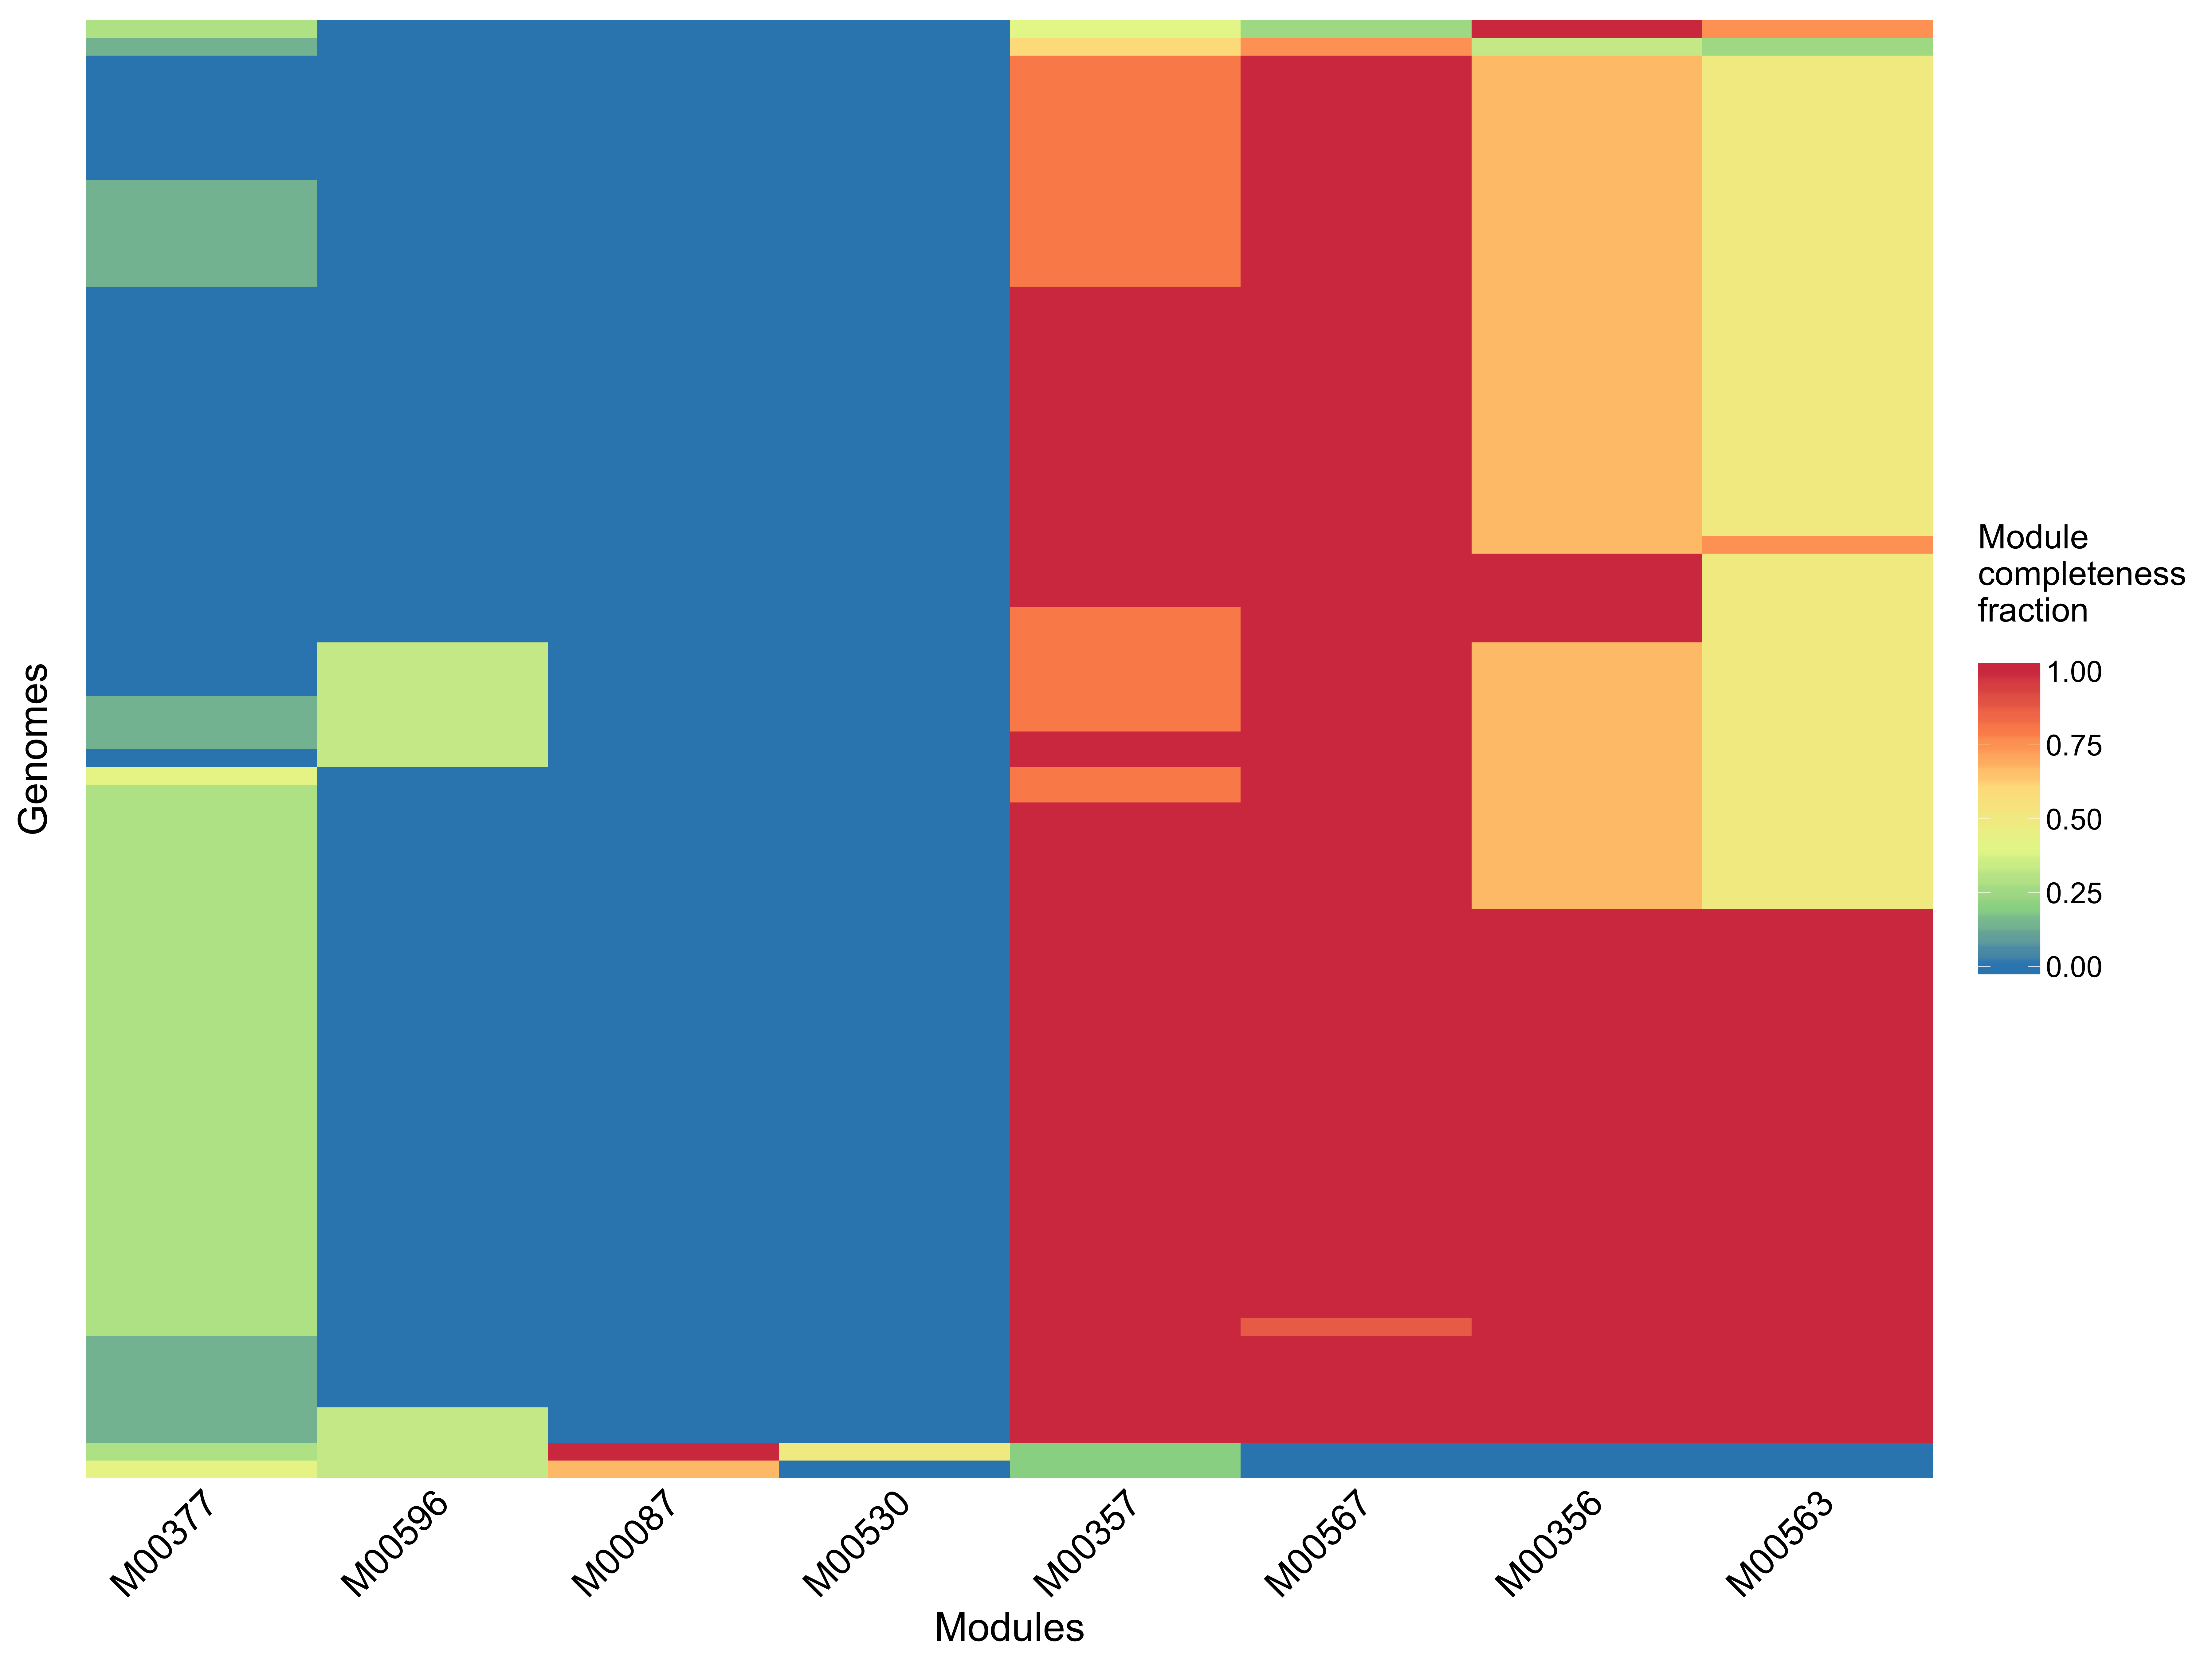
\includegraphics[width=0.85\textwidth]{module_allOrgs.png}
\caption{Module fraction presence across data sets}\label{fig:module_allOrgs.png}\end{figure}
\begin{figure}\centering
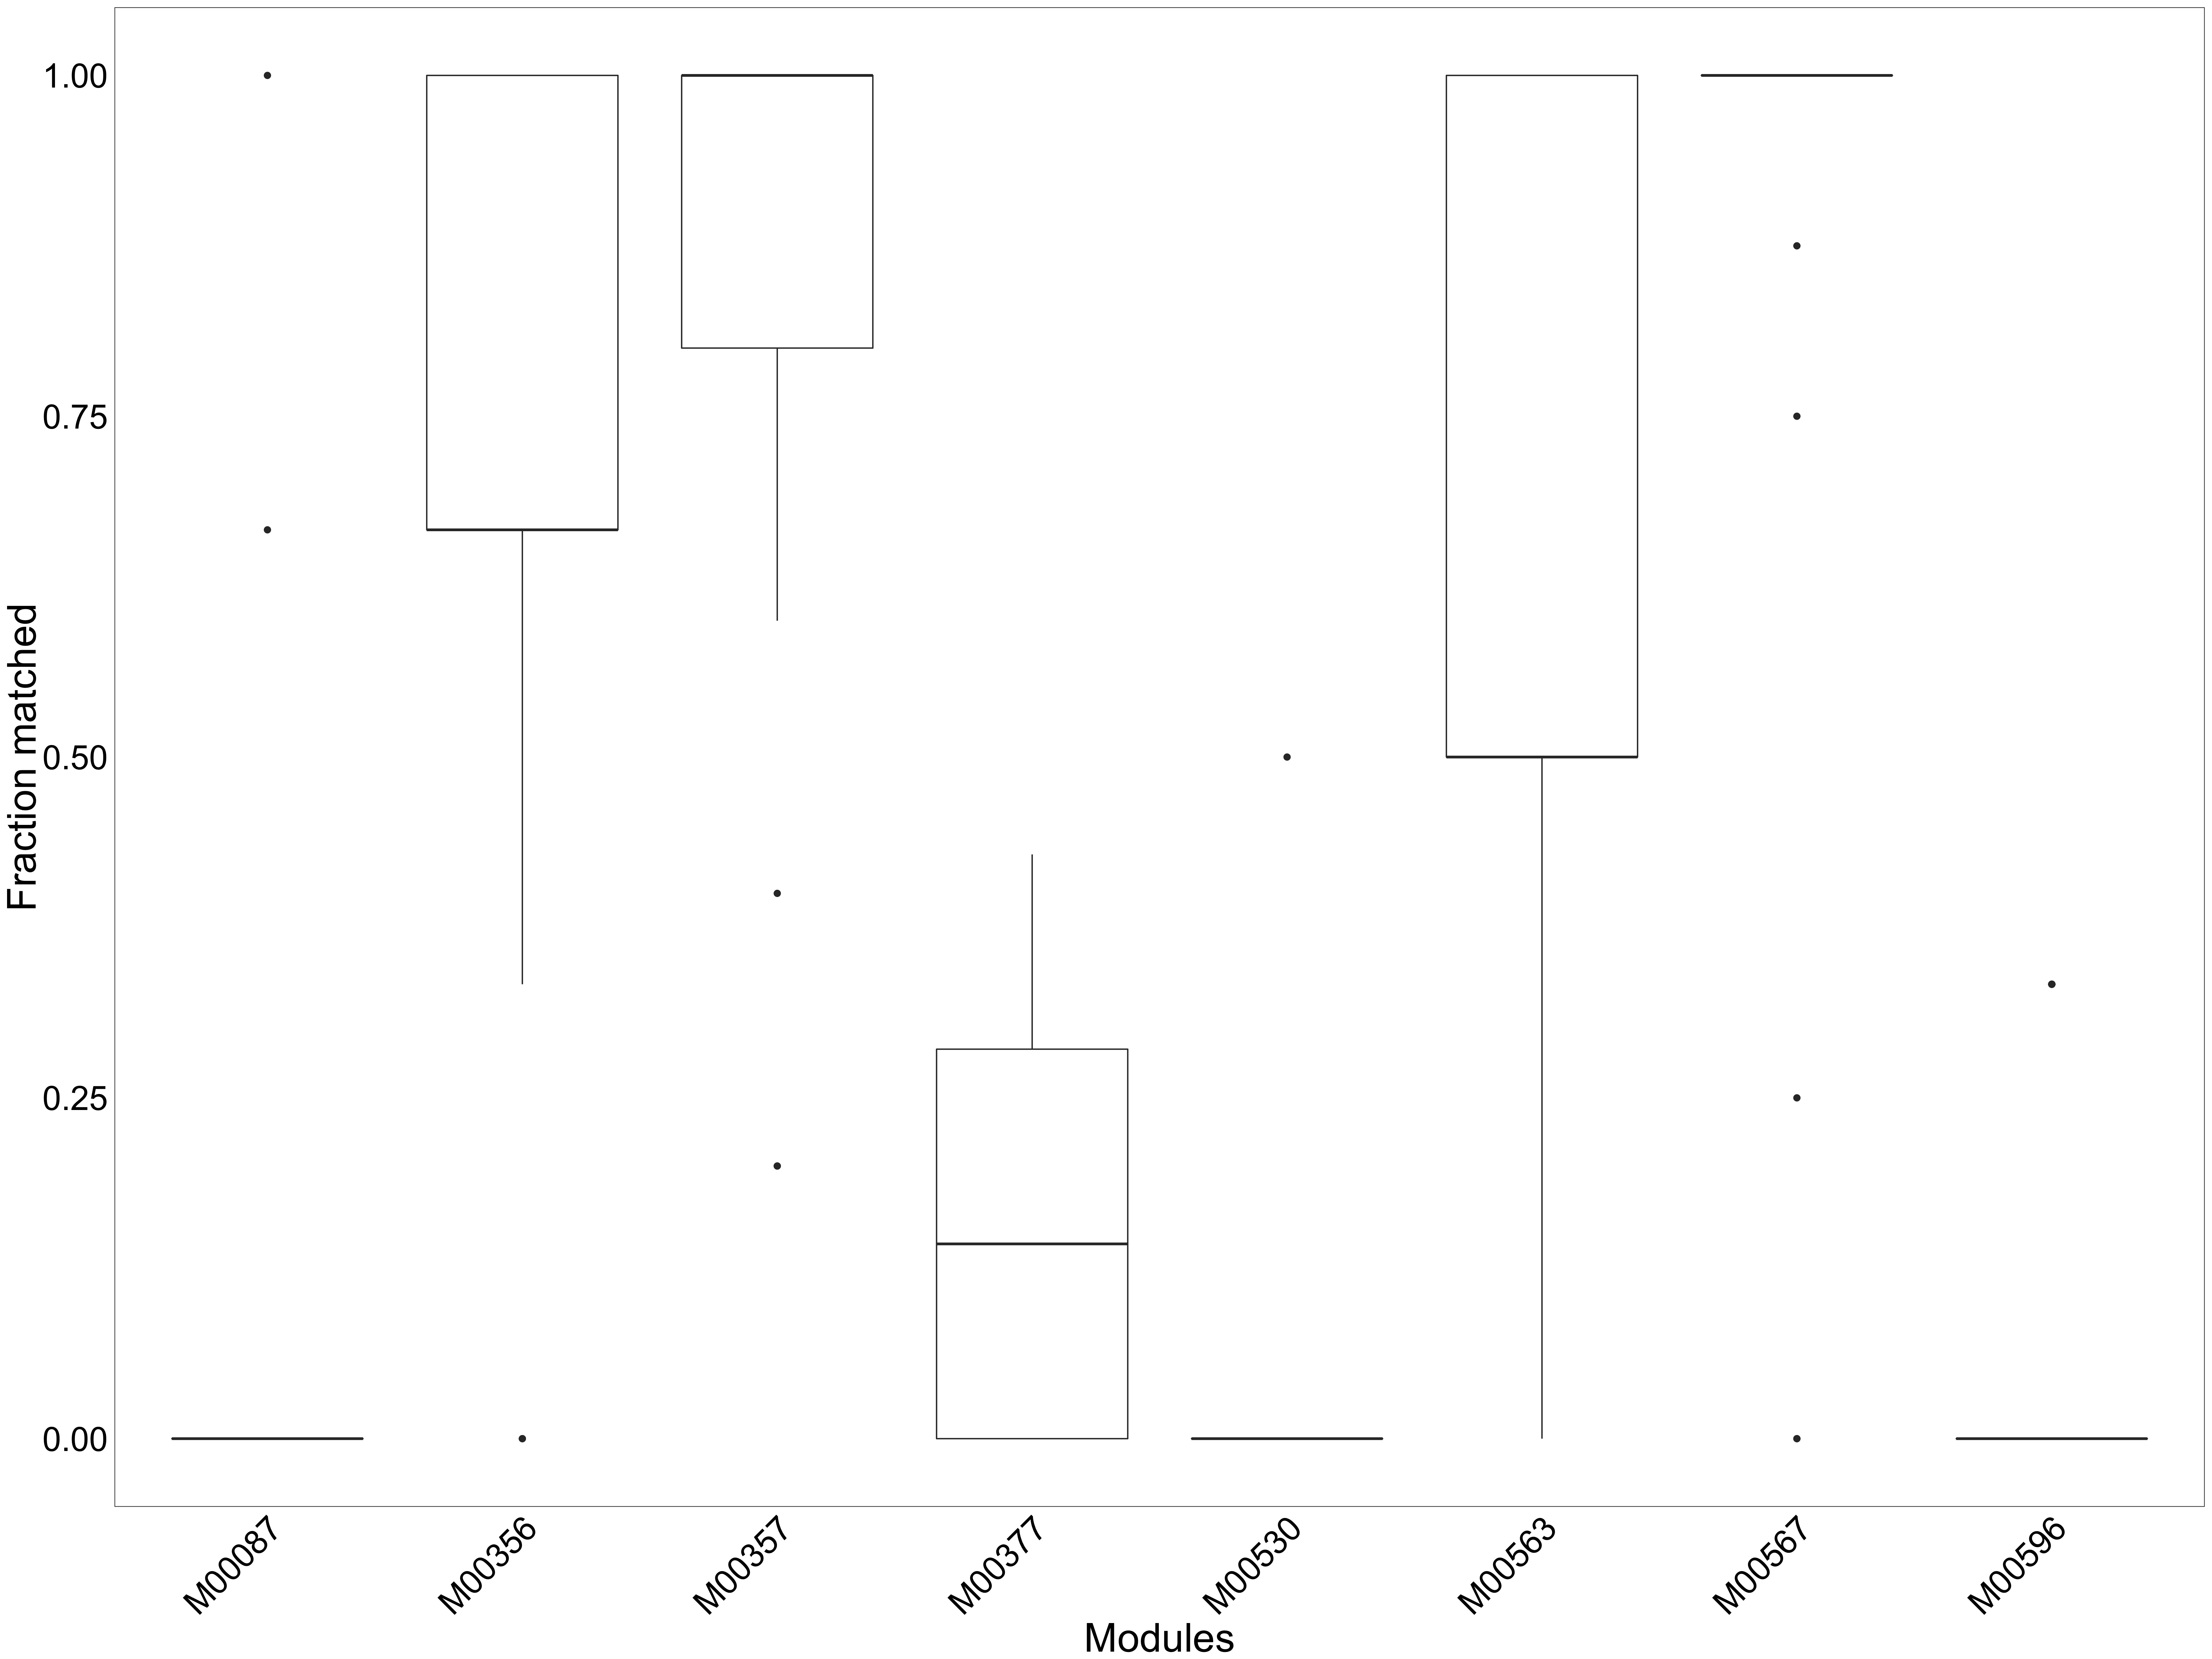
\includegraphics[width=0.85\textwidth]{module_allOrgs_sd_boxplot.png}
\caption{Module fraction presence variance - boxplot}\label{fig:module_allOrgs_sd_boxplot.png}\end{figure}
\begin{figure}\centering
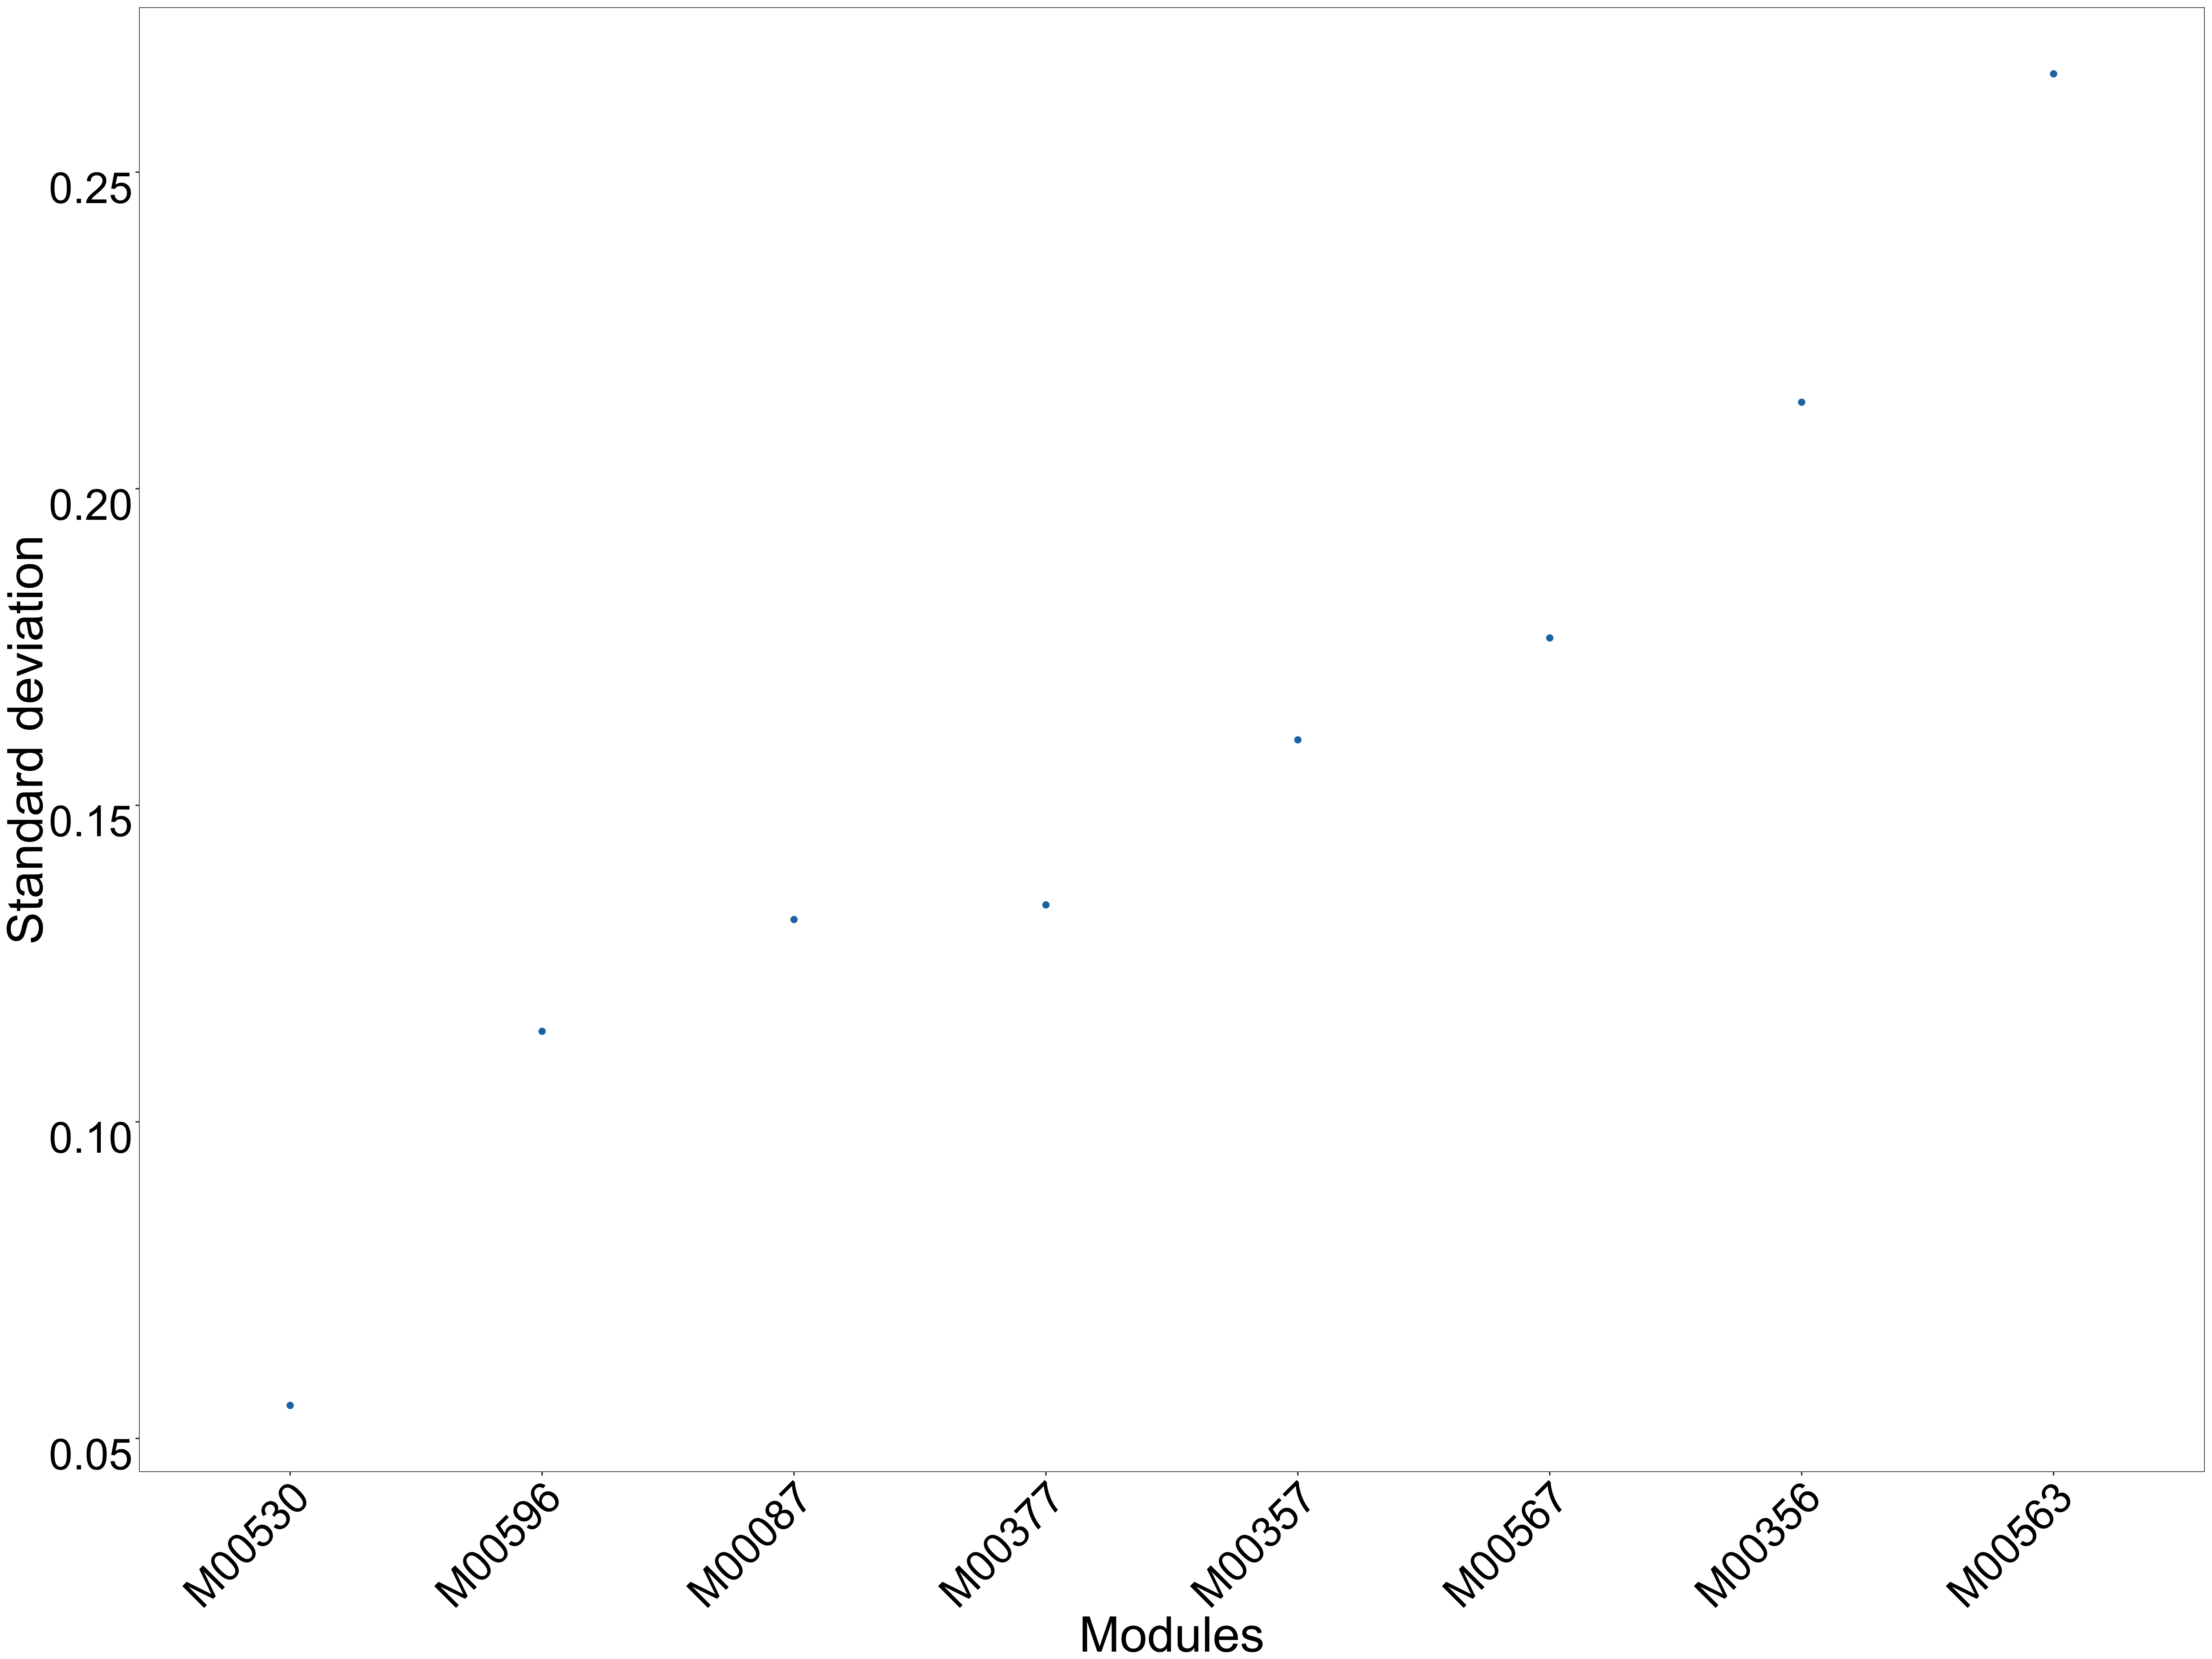
\includegraphics[width=0.85\textwidth]{module_allOrgs_sd.png}
\caption{Module fraction presence variance - scatter plot}\label{fig:module_allOrgs_sd.png}\end{figure}
\FloatBarrier
\subsubsection*{Module fraction presence: mean and variance by grouping factors}
\begin{figure}\centering
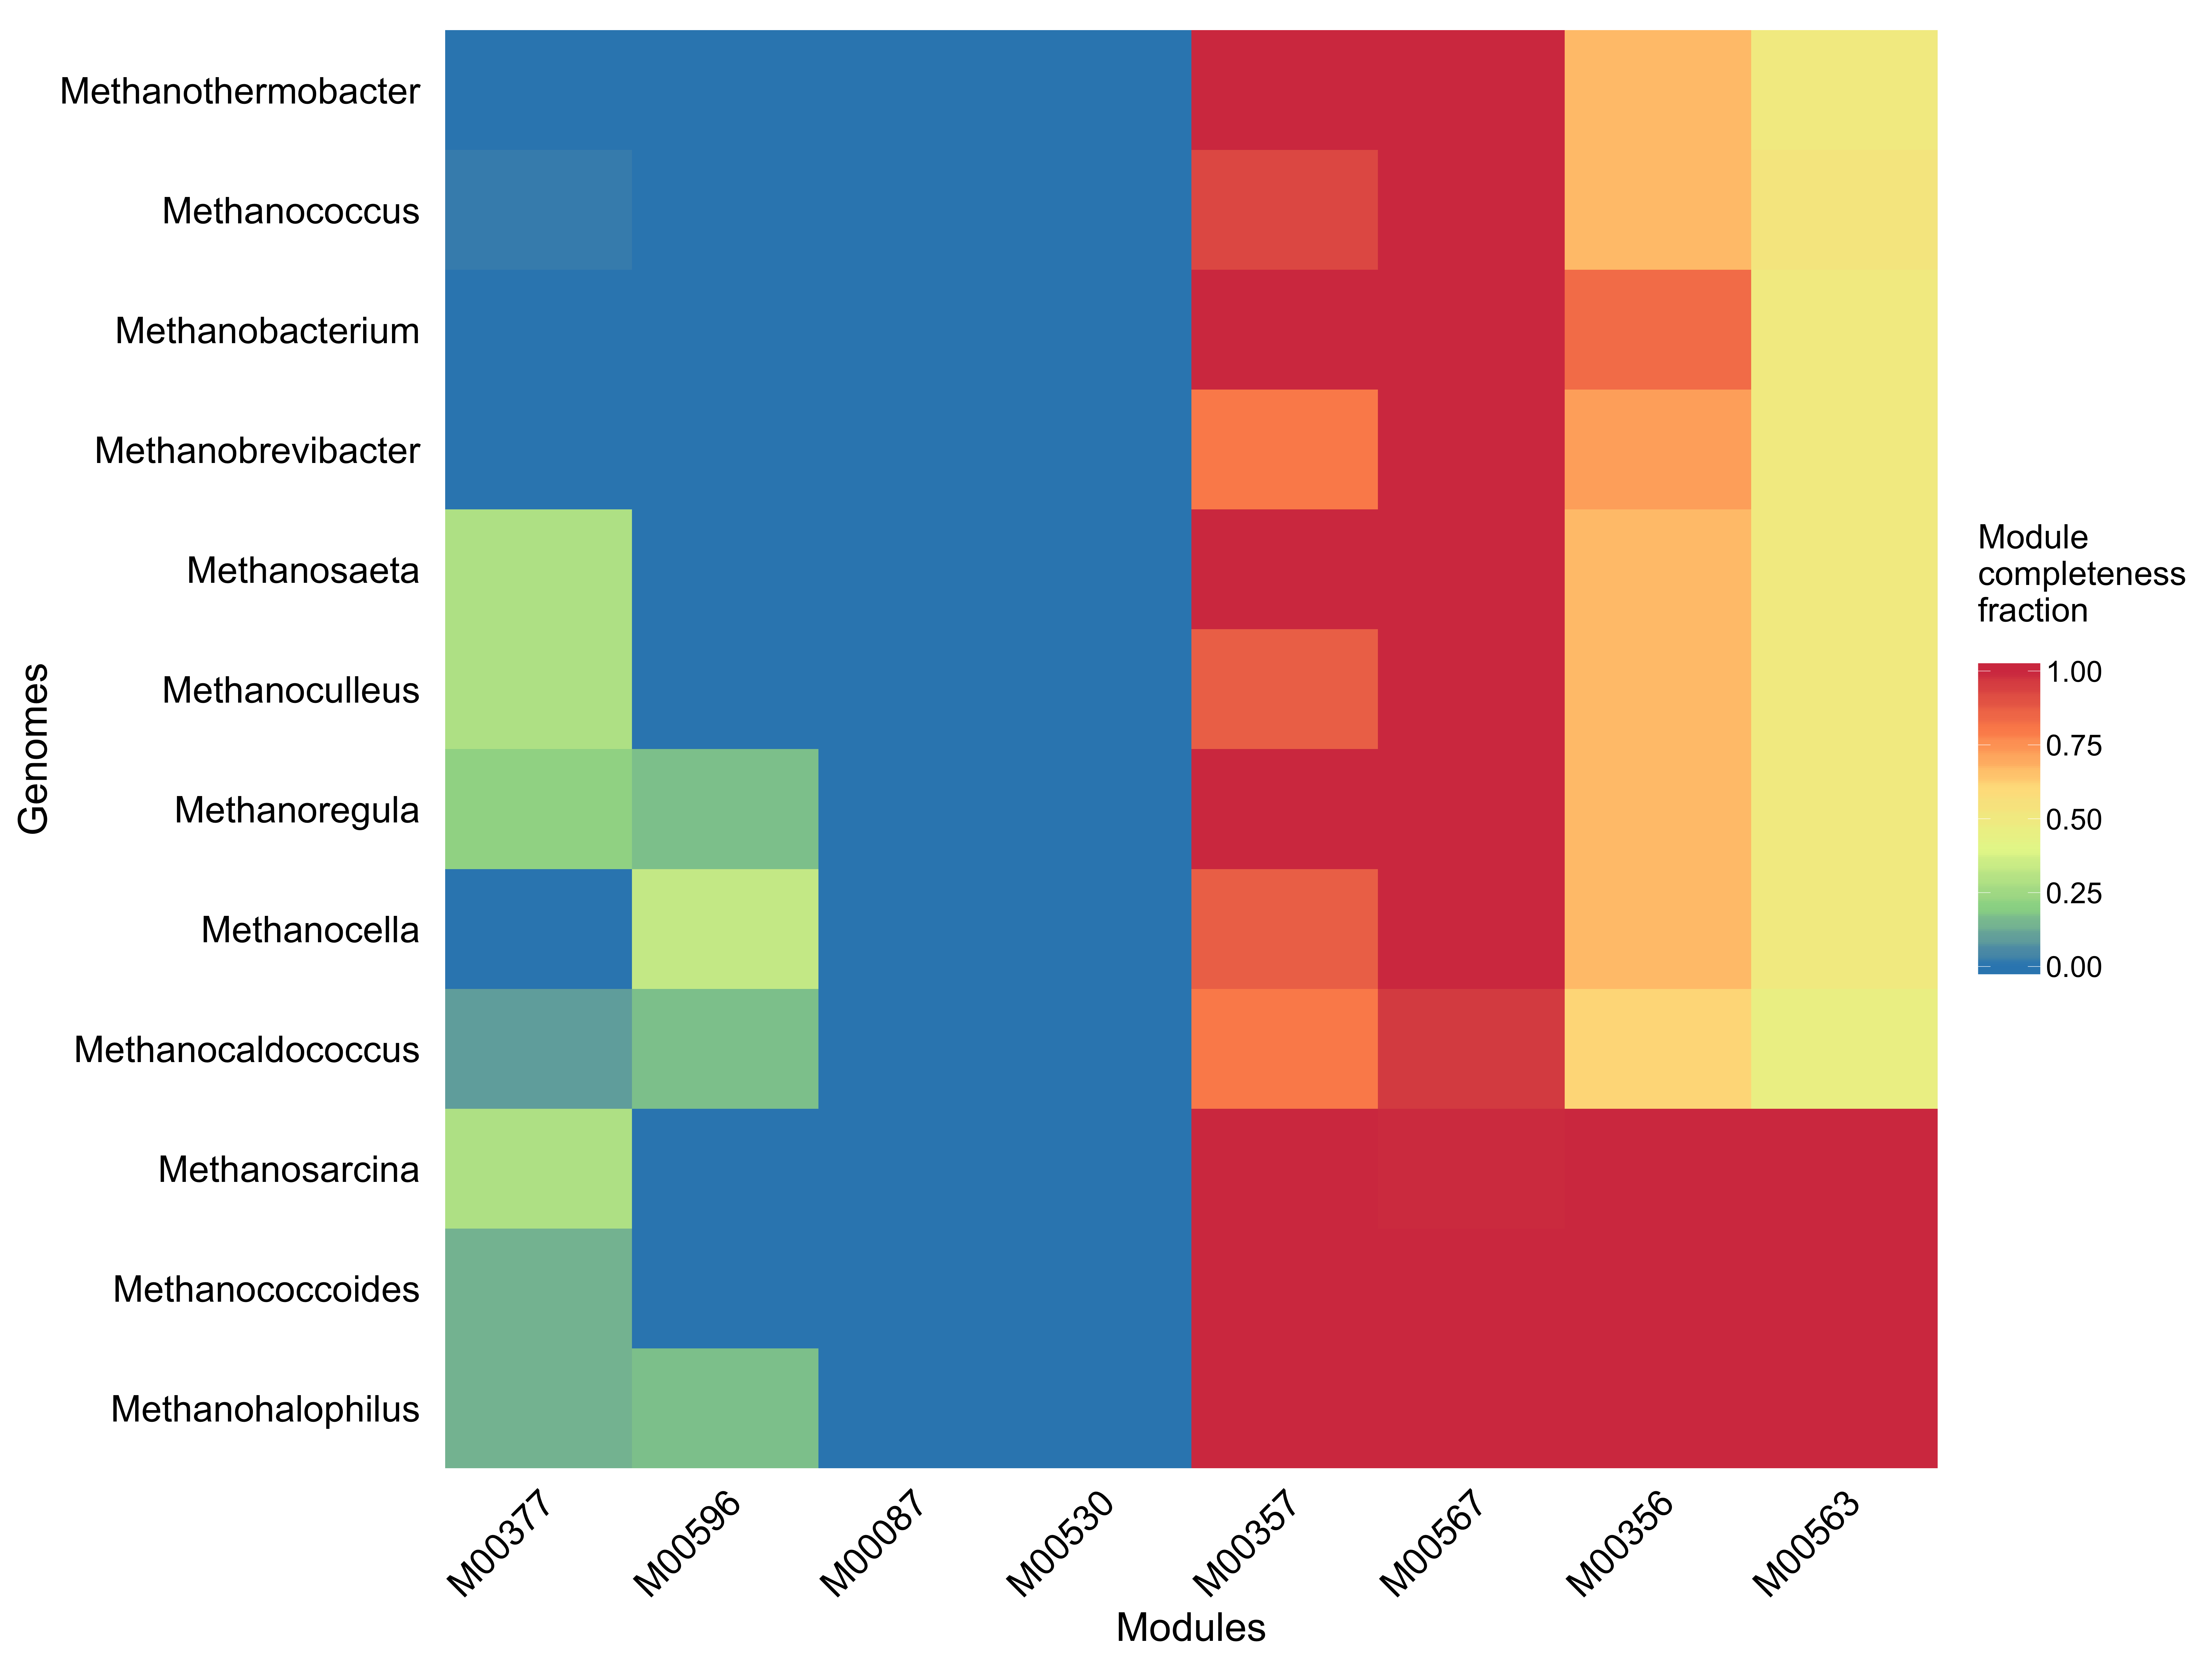
\includegraphics[width=0.85\textwidth]{module_mean_genusFactor.png}
\caption{genusFactor: mcf - mean}\label{fig:module_mean_genusFactor.png}\end{figure}
\begin{figure}\centering
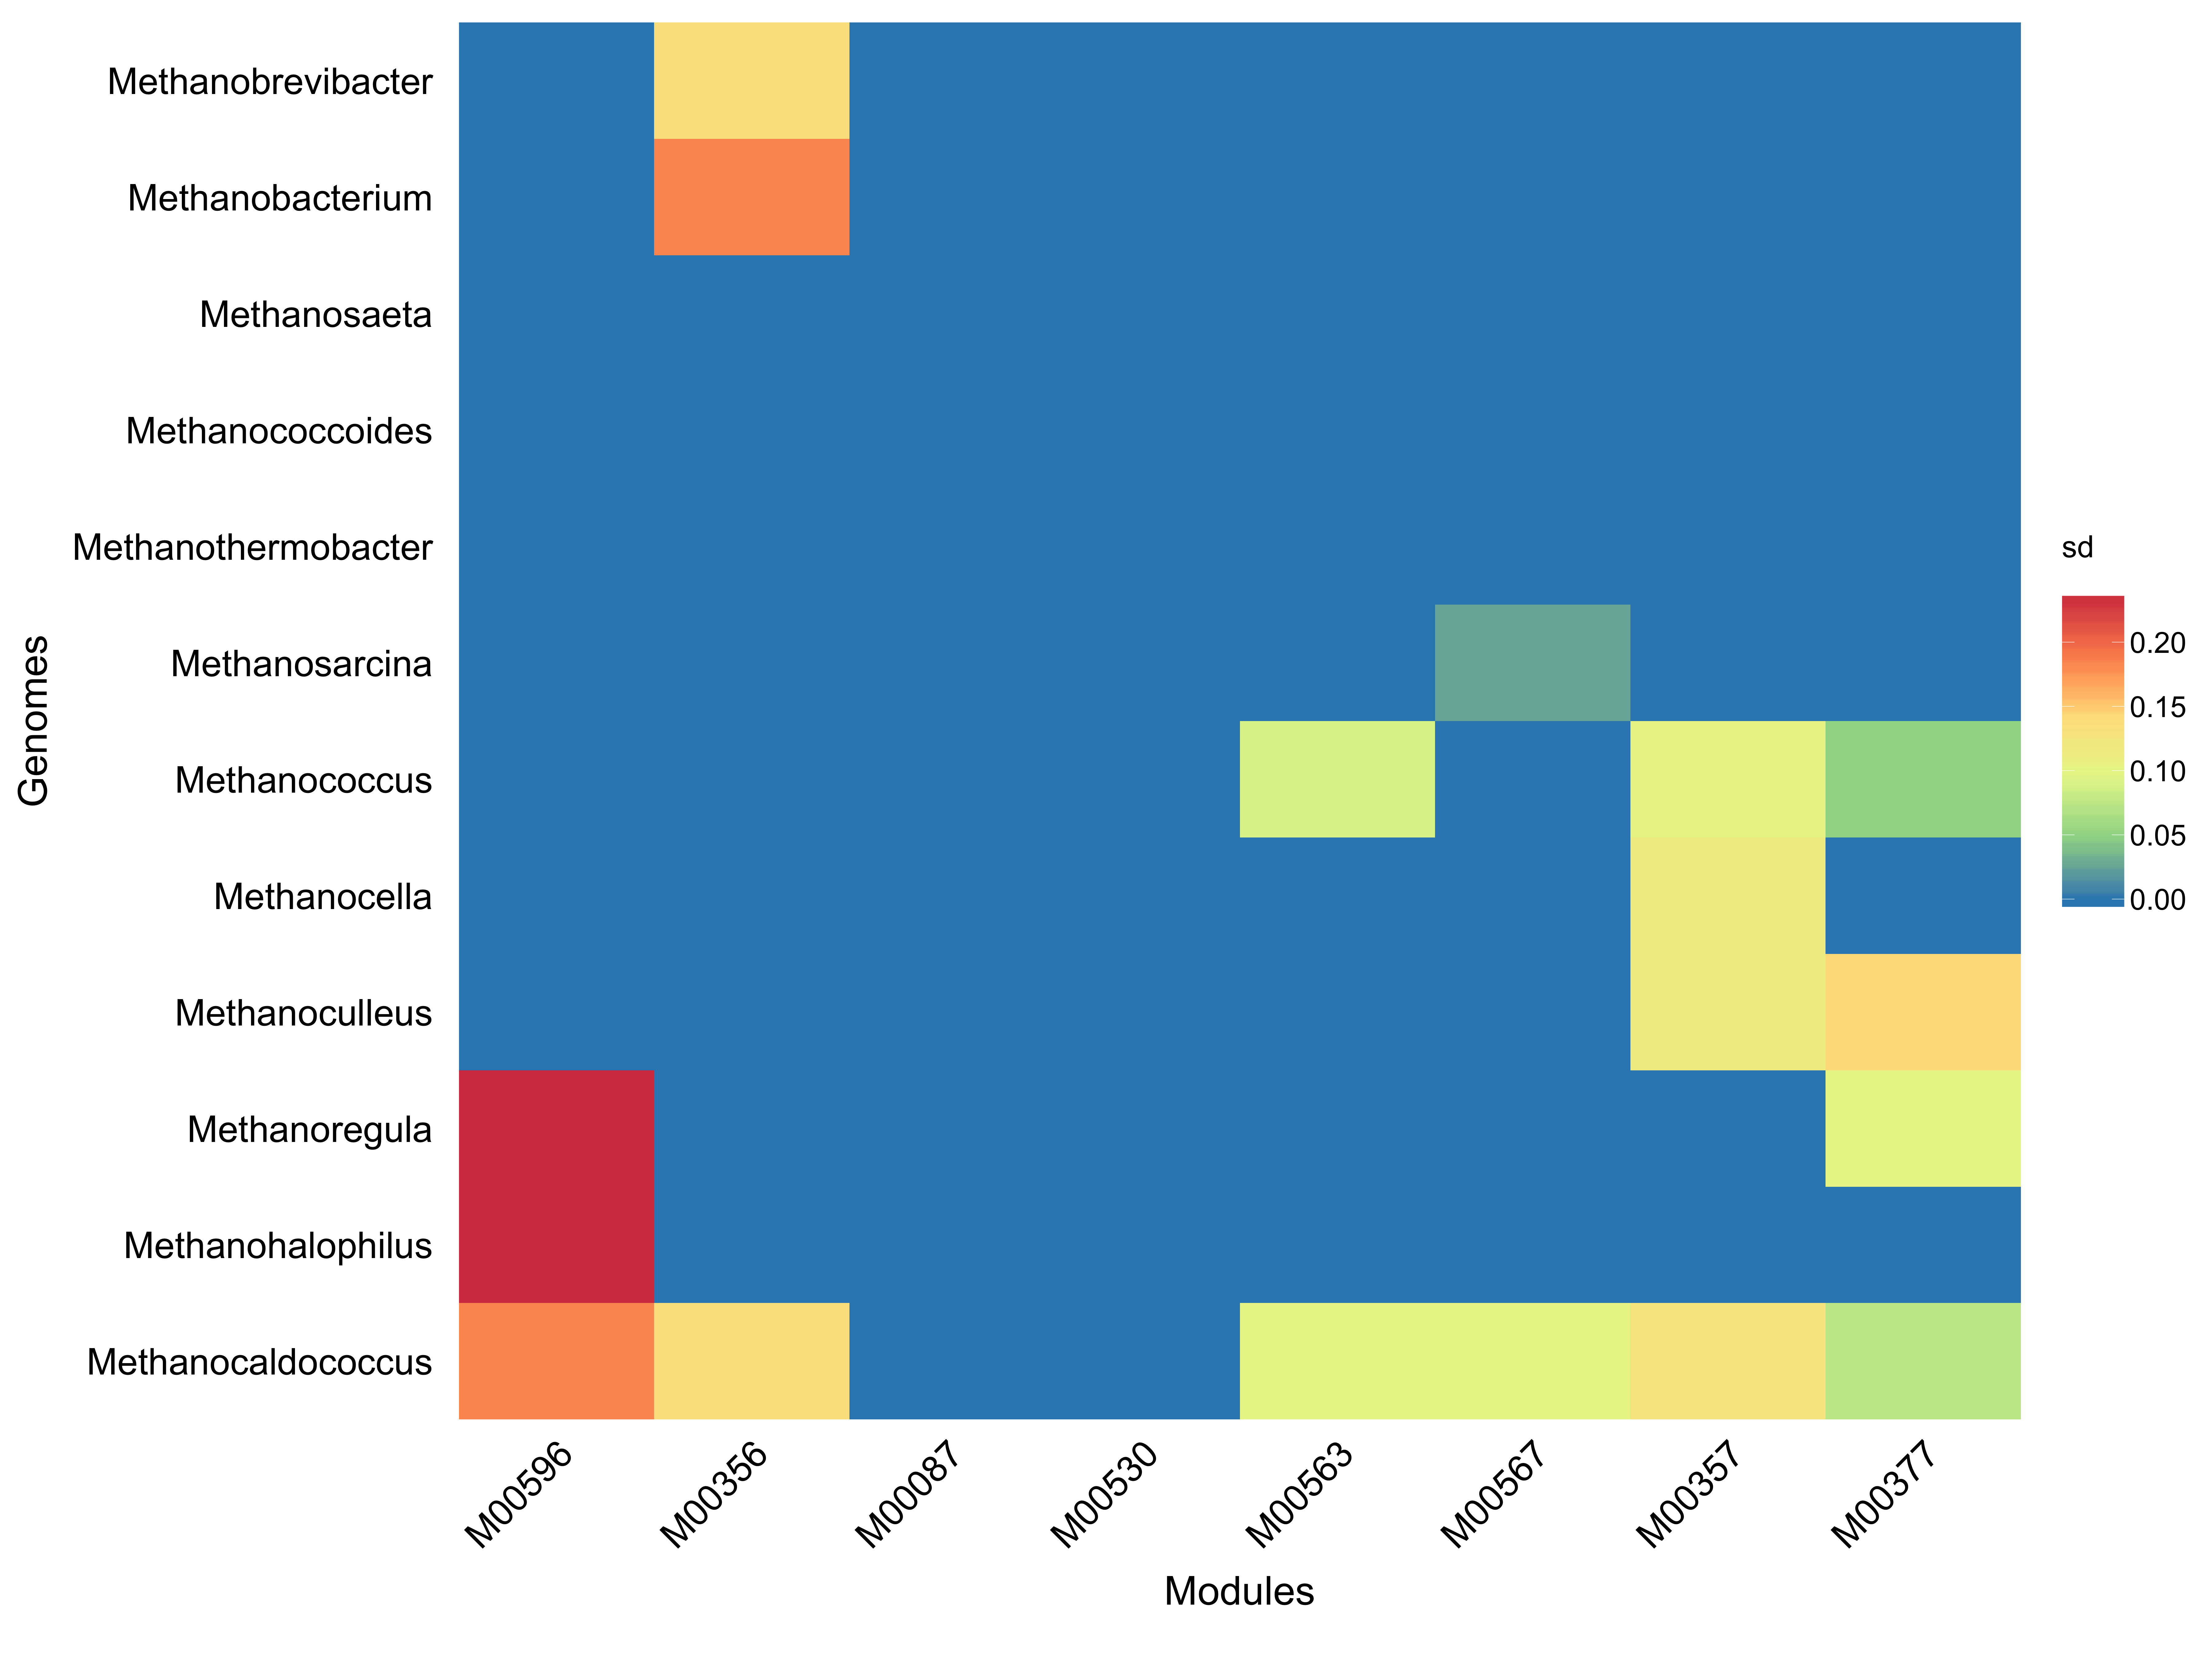
\includegraphics[width=0.85\textwidth]{module_sd_genusFactor.png}
\caption{genusFactor: mcf - standard deviation}\label{fig:module_sd_genusFactor.png}\end{figure}
No modules with zero variance.\\
\FloatBarrier
\subsection*{PCA}
PCA was done with the module analysis output.\\
\begin{figure}\centering
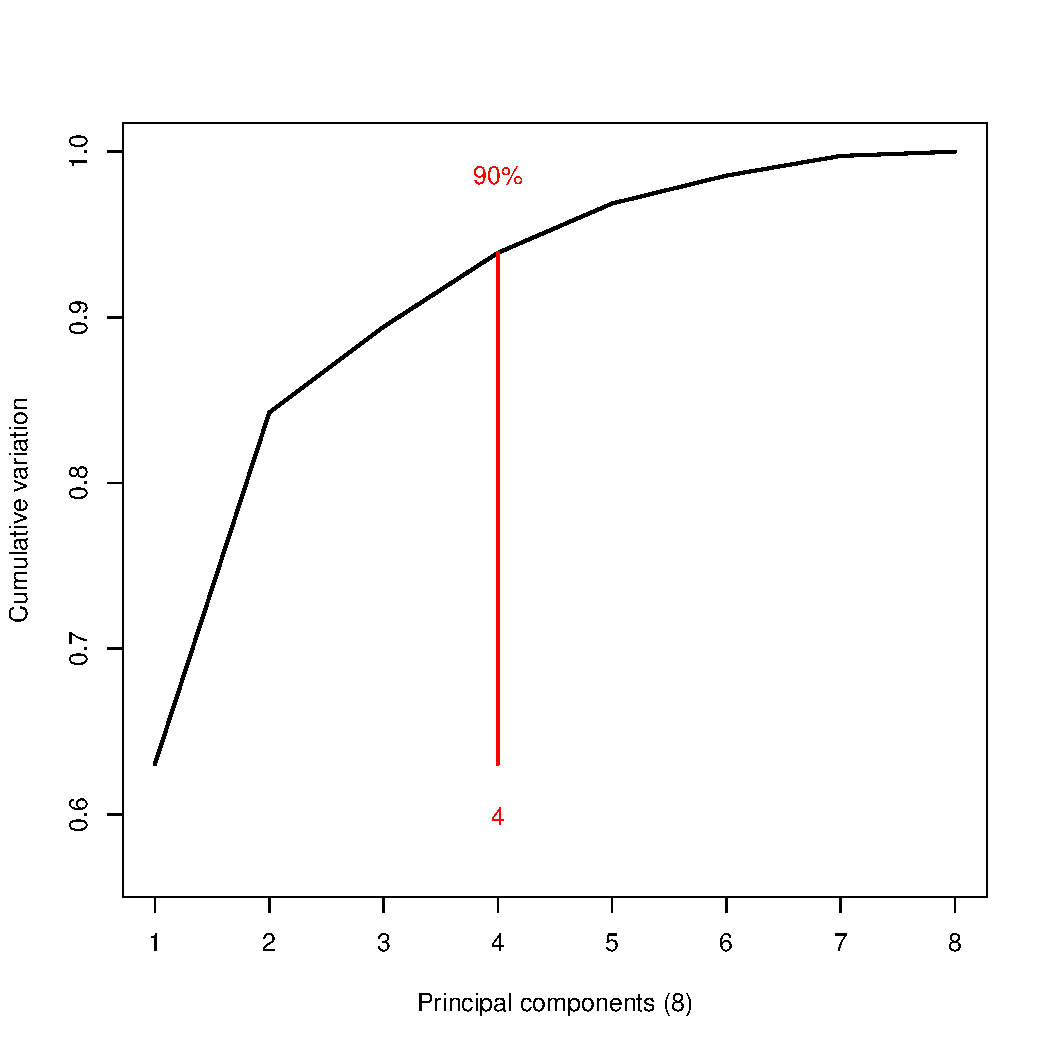
\includegraphics[width=0.85\textwidth]{PCA/pca_var.pdf}
\caption{Cumulative variance captured by principal components}\label{fig:PCA/pca_var.pdf}\end{figure}
\begin{figure}\centering
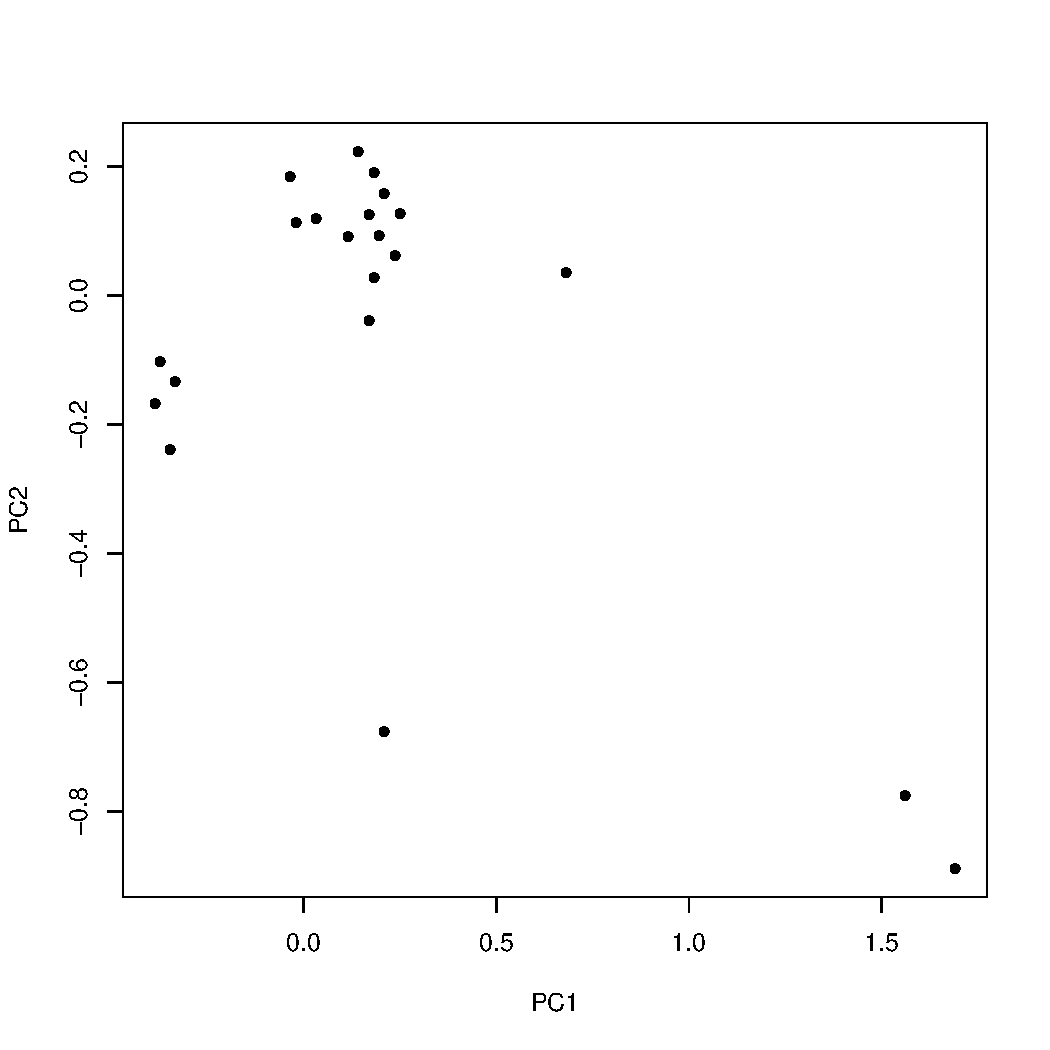
\includegraphics[width=0.85\textwidth]{PCA/pca_plot.pdf}
\caption{Princial component scatter plot}\label{fig:PCA/pca_plot.pdf}\end{figure}
Grouping ``factors'' were used to look at the data. The mean Euclidean distance ($m$) across the groups generated by factoring was calculated
    according to the following equation:
 \begin{equation} m =  \frac{\sum_i^N d_i}{N}\end{equation} where $N$ is the total number of distances between $p$ points, given by
      \begin{equation} N = \frac{p*(p-1)}{2} \end{equation}
 and are contained in the (module\_mean\_dist\_output\_FACTOR.rda object)\\
% latex table generated in R 3.4.1 by xtable 1.8-2 package
% Mon Mar  5 16:56:31 2018
\begin{table}[ht]
\centering
\begin{tabular}{lr}
  \hline
Factors & n\_Groups \\ 
  \hline
genusFactor & 27.00 \\ 
   \hline
\end{tabular}
\caption{Number of groups by factors} 
\label{tab:Factors}
\end{table}
\FloatBarrier
\subsubsection*{genusFactor}
\begin{figure}\centering
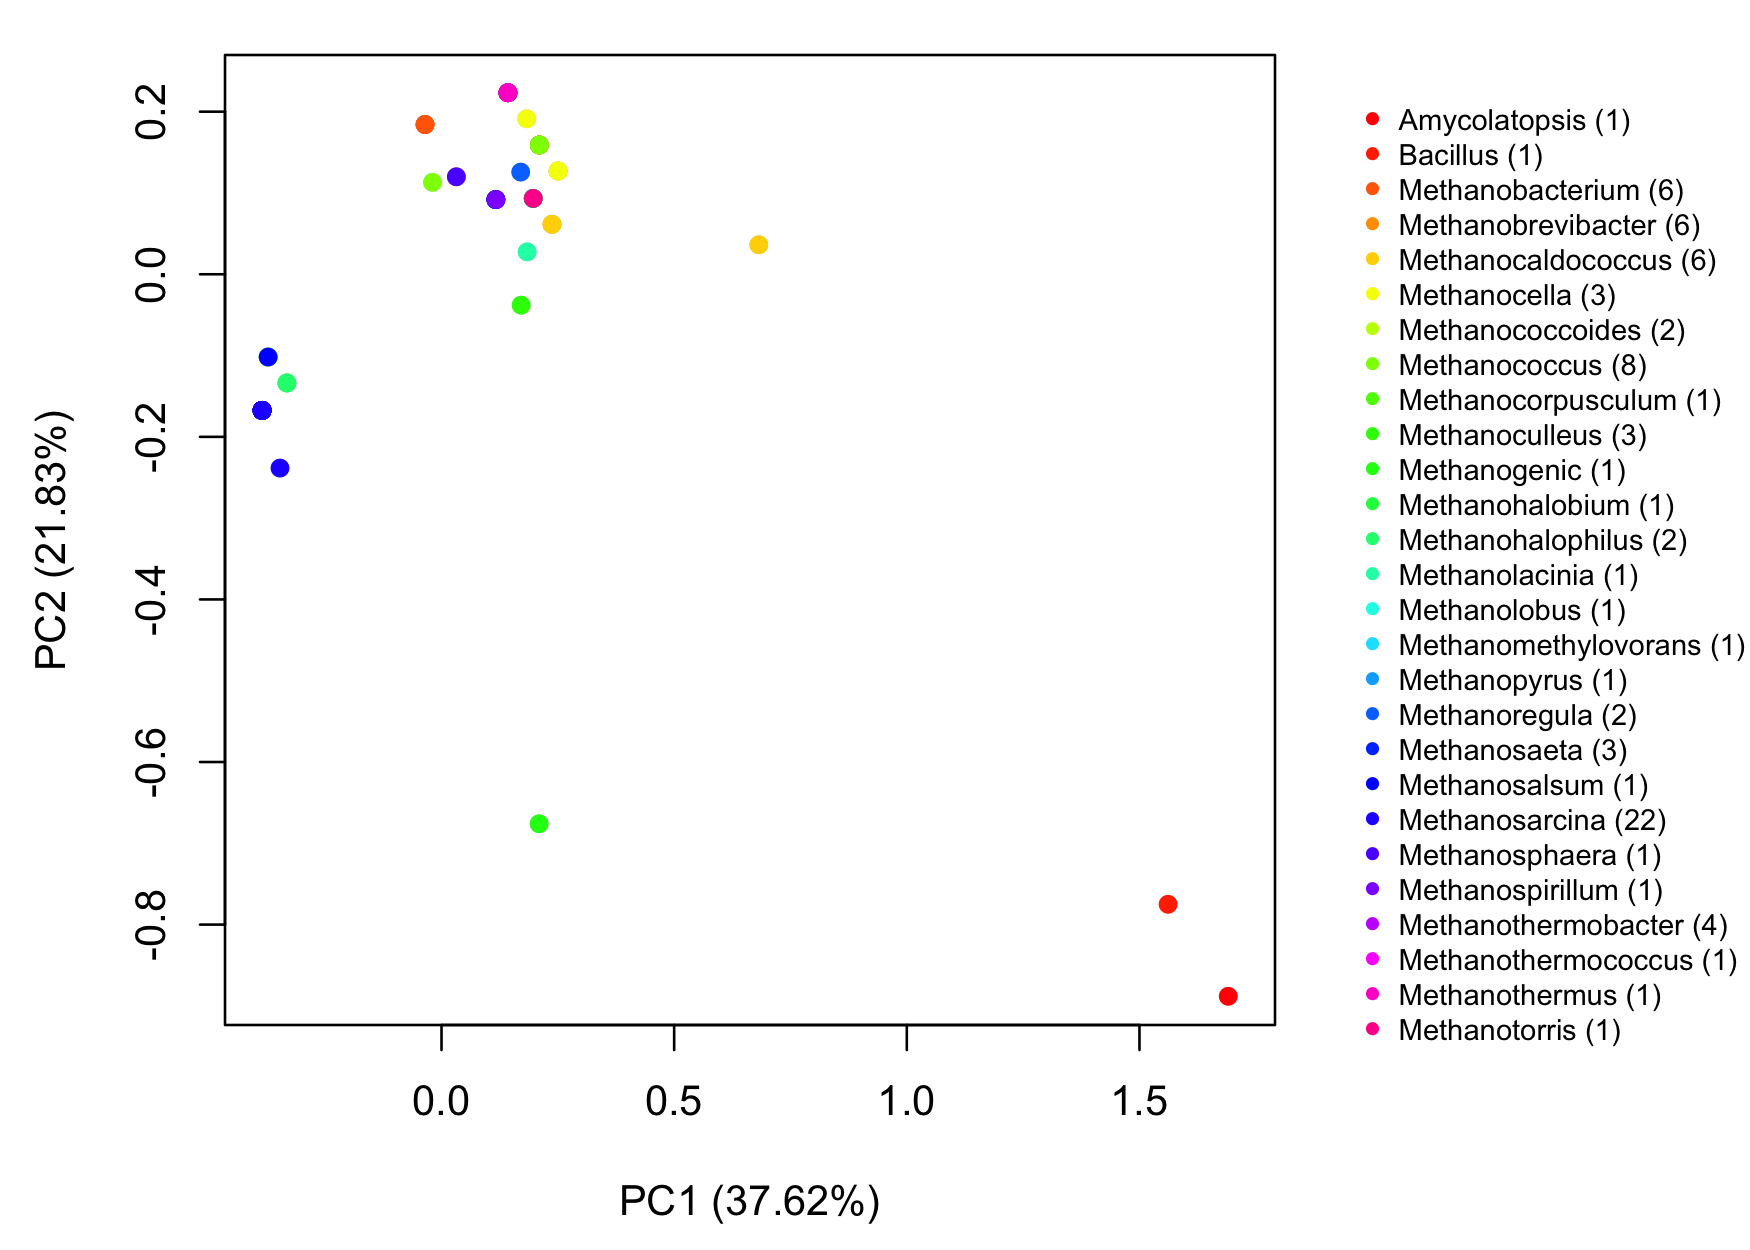
\includegraphics[width=0.85\textwidth]{PCA/plot_scatter_genusFactor.png}
\caption{genusFactor:  PC plot}\label{fig:PCA/plot_scatter_genusFactor.png}\end{figure}
\begin{figure}\centering
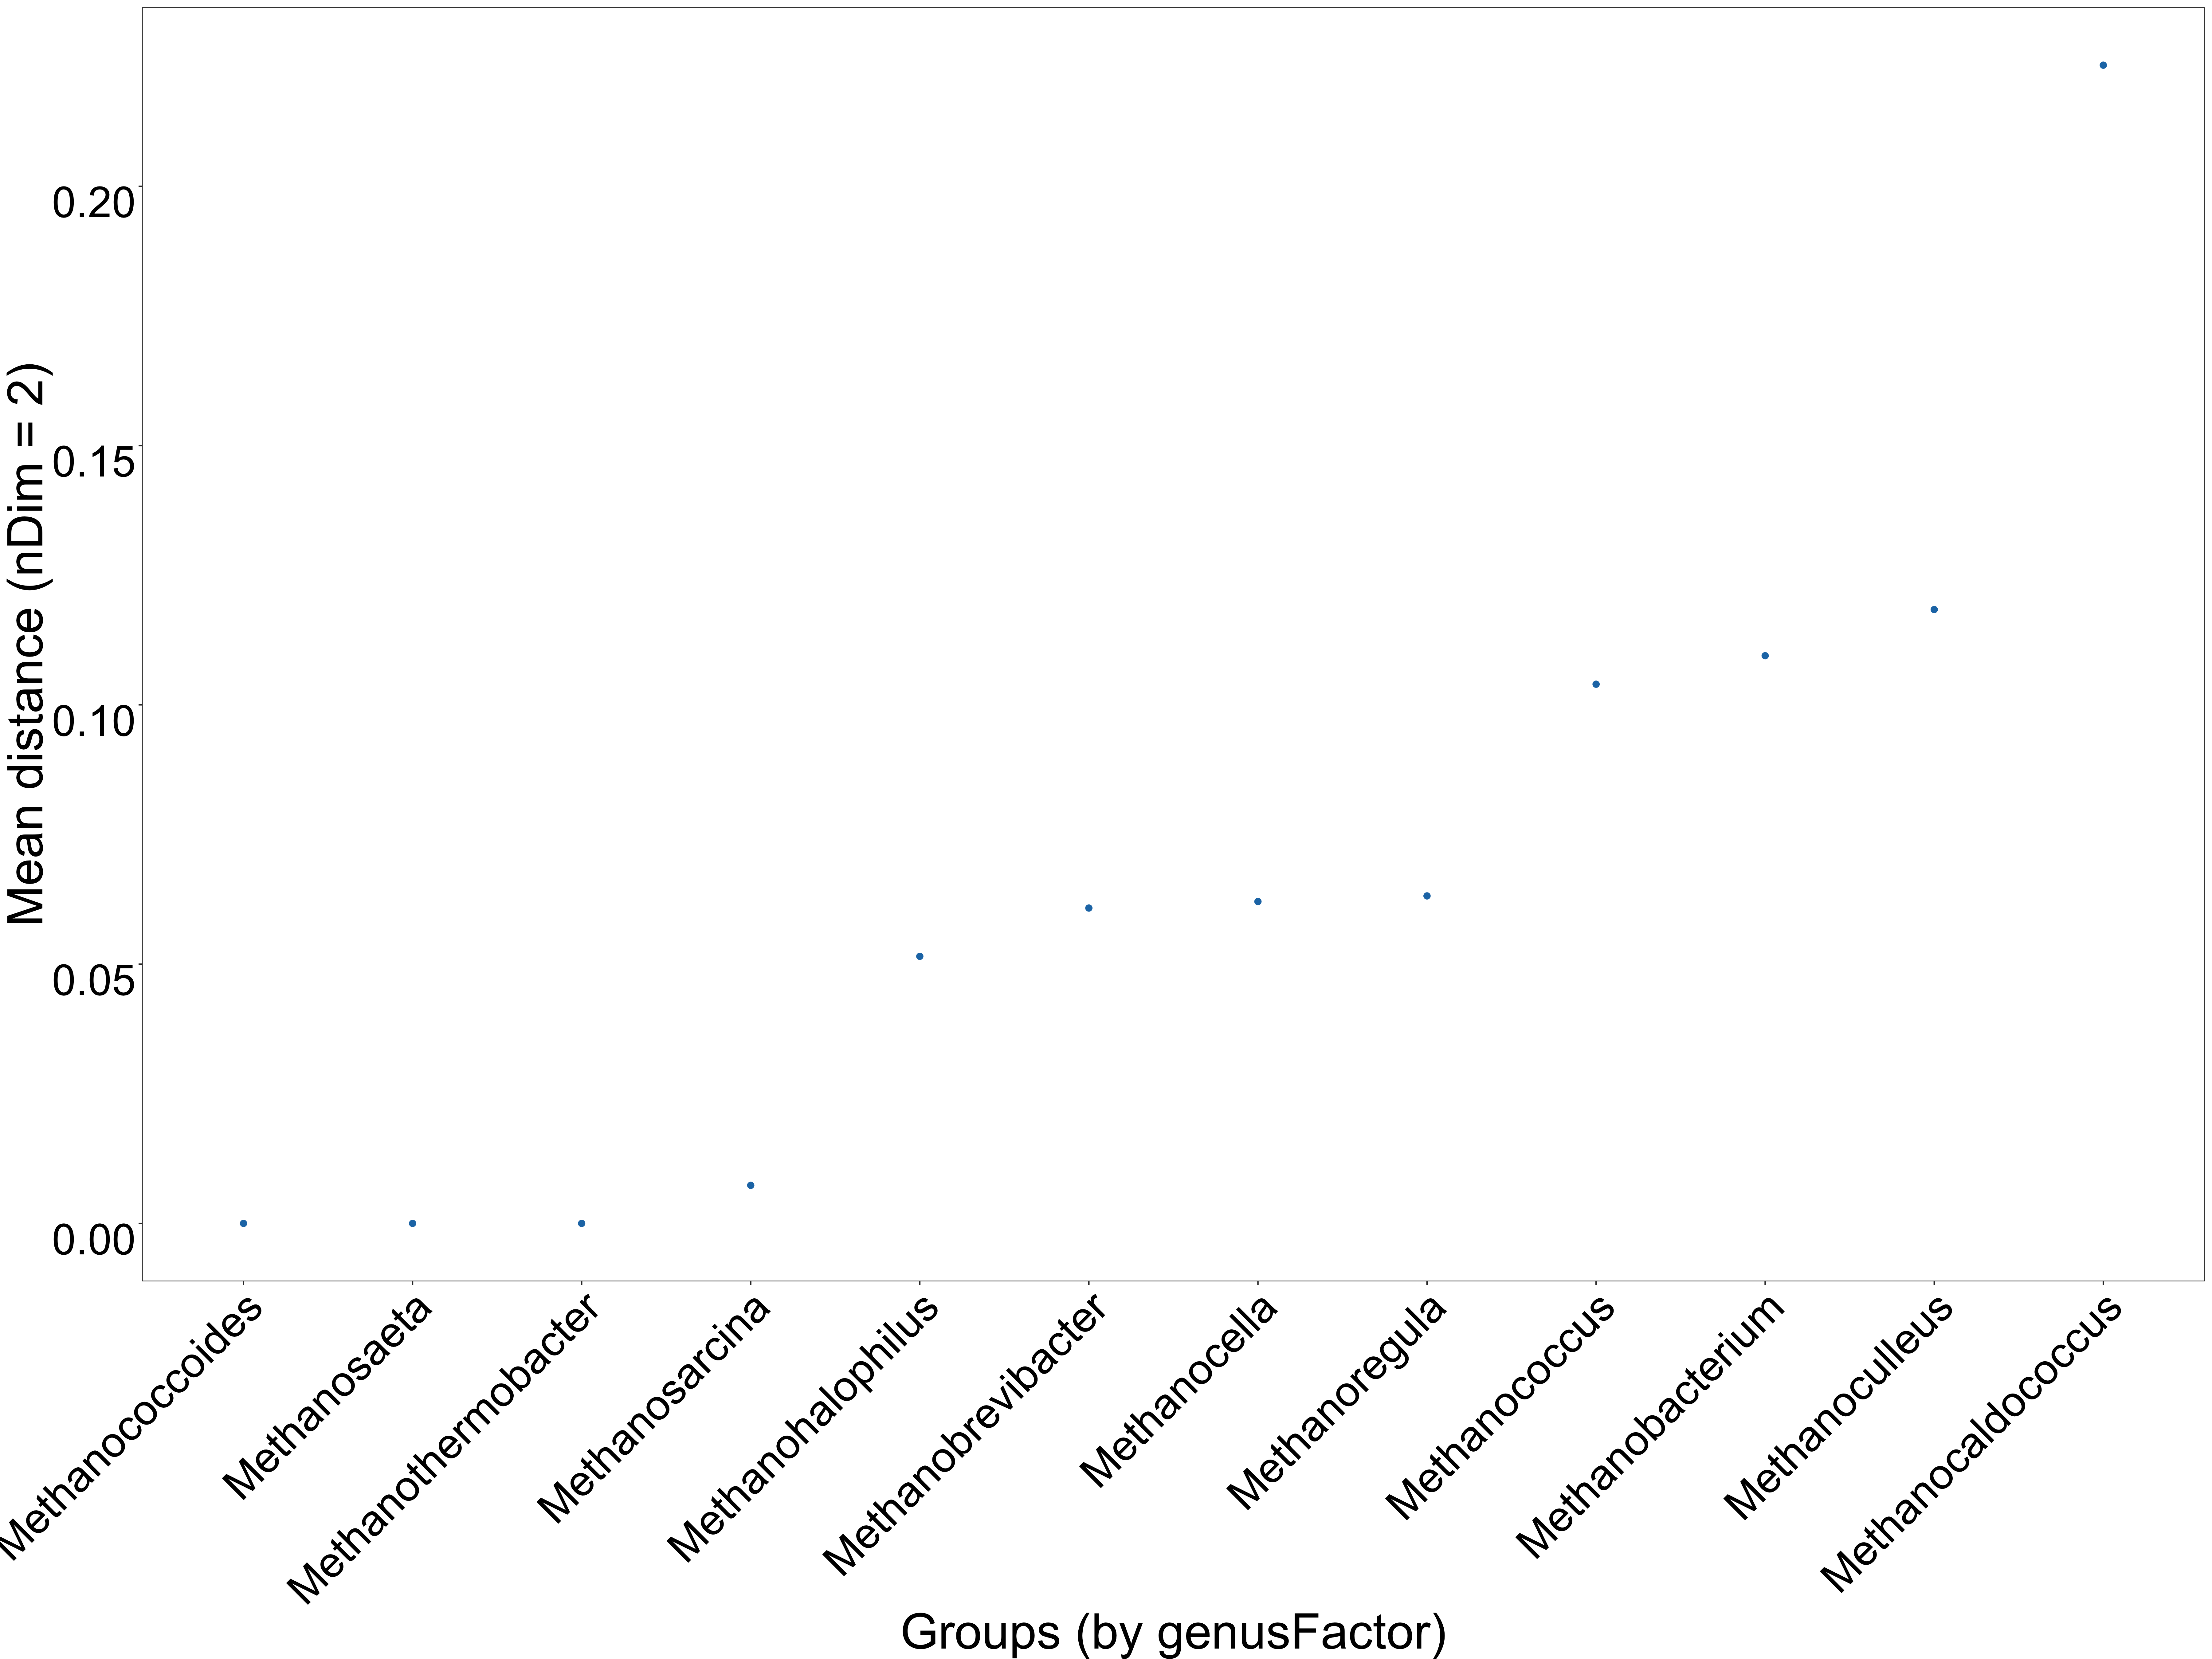
\includegraphics[width=0.85\textwidth]{PCA/plot_mean_dist_genusFactor.png}
\caption{genusFactor:  mean Euclidean distance}\label{fig:PCA/plot_mean_dist_genusFactor.png}\end{figure}
% latex table generated in R 3.4.1 by xtable 1.8-2 package
% Mon Mar  5 16:56:31 2018
\begin{table}[ht]
\centering
\begin{tabular}{lr}
  \hline
Groups & group\_counts \\ 
  \hline
Amycolatopsis & 1.00 \\ 
  Bacillus & 1.00 \\ 
  Methanobacterium & 6.00 \\ 
  Methanobrevibacter & 6.00 \\ 
  Methanocaldococcus & 6.00 \\ 
  Methanocella & 3.00 \\ 
  Methanococcoides & 2.00 \\ 
  Methanococcus & 8.00 \\ 
  Methanocorpusculum & 1.00 \\ 
  Methanoculleus & 3.00 \\ 
  Methanogenic & 1.00 \\ 
  Methanohalobium & 1.00 \\ 
  Methanohalophilus & 2.00 \\ 
  Methanolacinia & 1.00 \\ 
  Methanolobus & 1.00 \\ 
  Methanomethylovorans & 1.00 \\ 
  Methanopyrus & 1.00 \\ 
  Methanoregula & 2.00 \\ 
  Methanosaeta & 3.00 \\ 
  Methanosalsum & 1.00 \\ 
  Methanosarcina & 22.00 \\ 
  Methanosphaera & 1.00 \\ 
  Methanospirillum & 1.00 \\ 
  Methanothermobacter & 4.00 \\ 
  Methanothermococcus & 1.00 \\ 
  Methanothermus & 1.00 \\ 
  Methanotorris & 1.00 \\ 
   \hline
\end{tabular}
\caption{genusFactor} 
\label{tab:genusFactor}
\end{table}
\end{document}
